%
% 
%
%   2013/11/14  Ocean modeling ノート
%               河合 佑太
%
% style  Setting             %%%%%%%%
% フォント: 12point (最大), 片面印刷
\documentclass[a4j,12pt,openbib,oneside]{jreport}

%%%%%%%%%%%%%%%%%%%%%%%%%%%%%%%%%%%%%%%%%%%%%%%%%%%%%%%%
%%%%%%%%             Package Include            %%%%%%%%

\usepackage{ascmac}
\usepackage{tabularx}
\usepackage{graphicx}
\usepackage{amssymb}
\usepackage{amsmath}
\usepackage{mathrsfs}
\usepackage{framed}
\usepackage{wasysym}
\usepackage{wrapfig}
\usepackage{Dennou6}		% 電脳スタイル ver 6
%%%%%%%%%%%%%%%%%%%%%%%%%%%%%%%%%%%%%%%%%%%%%%%%%%%%%%%%
%%%%%%%%            PageStyle Setting           %%%%%%%%
\pagestyle{DAmyheadings}

%%%%%%%%%%%%%%%%%%%%%%%%%%%%%%%%%%%%%%%%%%%%%%%%%%%%%%%%
%%%%%%%%        Title and Auther Setting        %%%%%%%%
%%
%%  [ ] はヘッダに書き出される.
%%  { } は表題 (\maketitle) に書き出される.

\Dtitle{Ocean modeling ノート}   % 変更不可
\Dauthor{河合佑太}            % ゼミ担当者の名前
\Ddate{2013/11/14}        % ゼミの日時 (毎回変更すること)
\Dfile{fundamentals.tex}

%%%%%%%%%%%%%%%%%%%%%%%%%%%%%%%%%%%%%%%%%%%%%%%%%%%%%%%%
%%%%%%%%   Set Counter (chapter, section etc. ) %%%%%%%%
\setcounter{chapter}{0}    % 章番号
\setcounter{section}{0}    % 節番号
\setcounter{subsection}{1}    % 節番号
\setcounter{equation}{1}   % 式番号
\setcounter{page}{1}     % 必ず開始ページは明記する
\setcounter{figure}{1}     % 図番号
\setcounter{table}{0}      % 表番号
%\setcounter{footnote}{0}


%%%%%%%%%%%%%%%%%%%%%%%%%%%%%%%%%%%%%%%%%%%%%%%%%%%%%%%%
%%%%%%%%        Counter Output Format           %%%%%%%%
\def\thechapter{\arabic{chapter}}
\def\thesection{\arabic{chapter}.\arabic{section}}
\def\thesubsection{\arabic{chapter}.\arabic{section}.\arabic{subsection}}
\def\theequation{\arabic{chapter}.\arabic{section}.\arabic{equation}}
\def\thepage{\arabic{page}}
\def\thefigure{\arabic{chapter}.\arabic{section}.\arabic{figure}}
\def\thetable{\arabic{chapter}.\arabic{section}.\arabic{table}}
\def\thefootnote{*\arabic{footnote}}

%%%%%%%%%%%%%%%%%%%%%%%%%%%%%%%%%%%%%%%%%%%%%%%%%%%%%%%%
%%%%%%%%        Dennou-Style Definition         %%%%%%%%

%% 改段落時の空行設定
\Dparskip      % 改段落時に一行空行を入れる
%\Dnoparskip    % 改段落時に一行空行を入れない

%% 改段落時のインデント設定
\Dparindent    % 改段落時にインデントする
%\Dnoparindent  % 改段落時にインデントしない

%%%%%%%%%%%%%%%%%%%%%%%%%%%%%%%%%%%%%%%%%%%%%%%%%%%%%%%%%%
%% Macro defined by author
\def\univec#1{ \hat{ \Dvect{\rm #1}} }
\def\DPext#1#2#3{\left(\DP{#1}{#2} \right)_{#3}}

%%%%%%%%%%%%%%%%%%%%%%%%%%%%%%%%%%%%%%%%%%%%%%%%%%%%%%%%
%%%%%%%%             Text Start                 %%%%%%%%
\begin{document}
\chapter{海洋モデリング基礎}    % 章の始めからの場合はこのコマンドを使用する
%\section{順圧不安定}      % 節の始めからの場合はこのコマンドを使用する
\markright{\arabic{chapter}  海洋モデリング基礎 } %  節の題名を書き込むこと

%%%%%%%%%%%%%%%%%%%%%%%%%%%%%%%%%%%%%%%%%%%%%%%%%
\section{質量の連続の式}
\markright{\arabic{chapter}.\arabic{section} 質量の連続の式 } %  節の題名を書き込むこと


%%%%%%%%%%%%%%%%%%%%%%%%%%%%%%%%%%%%%%%%%%%%%%%%%
%%%%%%%%%%%%%%%%%%%%%%%%%%%%%%%%%%%%%%%%%%%%%%%%%
\section{運動量方程式}
\markright{\arabic{chapter}.\arabic{section} 運動量方程式 } %  節の題名を書き込むこと
%%%%%%%%%%%%%%%%%%%%%%%%%%%%%%%%%%%%%%%%%%%%%%%%%
%%%%%%%%%%%%%%%%%%%%%%%%%%%%%%%%%%%%%%%%%%%%%%%%%
\section{状態方程式}
\markright{\arabic{chapter}.\arabic{section} 状態方程式 } %  節の題名を書き込むこと
三次元において, 運動量方程式と連続の式は四本の方程式を与えるが, 五個の未知変数(速度の三成分, 密度, 圧力)を含む. 
明らかに他の方程式が必要とされる. 
そして, \textbf{状態方程式}(equation of state)が, 診断的にさまざまな熱力学変数を互いに関係付ける式である. 
\textbf{習慣的な}状態方程式(熱的状態方程式(thermal equation of state)とも呼ばれる)は, 
温度,圧力,成分(さまざま構成物質の質量分率), 密度を関係付ける. 
これは, 一般的には
\begin{equation}
 p = p(\rho, T, \mu_n)
\end{equation}
と書かれる. 
ここで, $\mu_n$は$n$番目の構成物質の質量分率である. 
この形式の方程式は, 熱力学的な観点からは最も基本的な状態方程式ではない. 
しかし, 習慣的な状態方程式は, 簡単に計測できる量を結びつける. 

理想気体(地球大気は理想気体にとても近い)に対する習慣的な状態方程式は, 
\begin{equation}
 p = \rho R T 
 \label{eq:conventionalEOS_forIdealGas}
\end{equation}
である. 
ここで, $R$は考えれる気体の気体定数, $T$は温度である. 
($R$は, 万有気体定数$R_u$と$R = R_u/m$によって関係付けられる. ここで, $m$は気体成分の平均分子量である. 
また, $R=nk$でもある. ここで, $k$はボルツマン定数, $n$は単位質量あたりの分子数である.)
乾燥空気に対して, $R=287$J kg$^{-1}$ K$^{-1}$である. 
空気は, 水蒸気量の変化を除けば, 仮想的に一定の成分を持つ. 
水蒸気量の指標は, 水蒸気混合比$w=\rho_w/\rho_d$である. 
ここで, $\rho_w, \rho_d$はそれぞれ水蒸気と乾燥空気の密度である. 
大気では, $w$は 0 から 0.03 の間を変化する. 
この変化は, 状態方程式中の気体定数を, 水蒸気混合比の弱い関数にする. 
つまり, $p = \rho R_{\rm eff} T$、 
ここで, $R_{\rm eff}=R_d ( 1+ w R_v/R_d)/(1+w)$であり, 
$R_d$, $R_v$はそれぞれ乾燥空気, 水蒸気に対する気体定数である. 
$w \sim 0.01$なので, $R_{\rm eff}$の変化は極めて小さく, 理論的研究ではしばしば無視される. 

海水のような流体に対しては, (\ref{eq:conventionalEOS_forIdealGas})と類似した簡潔な表現は簡単には導けない. 
そのため, 半経験則的な方程式がふつう用いられる. 
実験室の設定における純粋では, 状態方程式の妥当な近似は, $\rho = \rho_0 [1 - \beta_T(T-T_0)]$である. 
ここで, $\beta_T$は熱膨張係数, $\rho_0,T_0$は定数である. 
海洋では, 密度は, 圧力と溶解した塩によって重要な影響を受ける. 
海水は, 水の中にたくさんのイオンが溶解している溶液であり, 
塩化物(質量で$\approx 1.9\%$), ナトリウム($1\%$), 硫化物($0.26\%$), マグネシウム($0.13\%$), その他が含まれ,  
これらの全平均的な濃度は$35 \permil$である. 
これらの塩の割合は, 海洋を通して多かれ少なかれ一定であり, 
全濃度は一つの指標, \textbf{塩分}(salinity)$S$によってパラーメタ化される. 
これにより, 海水の密度は三個の変数(圧力, 温度, 塩分)の関数である. 
そして, 海水の習慣的な状態方程式は, 
\begin{equation}
 \alpha = \alpha (T,S,p)
\end{equation}
と書かれる. 
ここで, $\alpha=\rho^{-1}$は比容で, 密度の逆数である. 
参照値付近の小さな変動に対し, 
\begin{equation}
\begin{split}
 d\alpha &= \DP[][S,p]{\alpha}{T} dT + \DP[][T,p]{\alpha}{S} dS + \DP[][T,S]{\alpha}{p} dp \\
         &= \alpha (\beta_T dT - \beta_S dS - \beta_p dp)
\end{split}
\end{equation}
ここで, 最後の式は, 熱膨張率$\beta_T$, 塩分圧縮係数$\beta_S$,  
圧縮係数(体積弾性係数の逆数)$\beta_p$を定義する. 
一般には, これらの量は定数でないが, 参照値の周りの小さな変化に対しては, 
定数と取り扱ってよいだろう. 
このとき, 
\begin{equation}
 \alpha = \alpha_0 \left[ 1 + \beta_T(T-T_0) - \beta_S(S-S_0) - \beta_p (p-p_0) \right]
 \label{eq:conventionLinearEOS_specVol_forSeaWater}
\end{equation}
を得る. 
これらのパラメータの典型的な値は, 海洋でよく見かける変動量も含めて, 
$\beta_T \approx 2(\pm 1.5) \times 10^{-4} $ K$^{-1}$(値は温度・圧力ともに一緒に増加する), 
$\beta_S \approx 7.6(\pm 0.2) \times 10^{-4}$ ppt$^{-1}$, 
$\beta_p \approx 4.1(\pm 0.5) \times 10^{-10}$ Pa$^{-1}$である. 
平均的な密度近傍の変化は小さいので, (\ref{eq:conventionLinearEOS_specVol_forSeaWater})から, 
\begin{equation}
 \rho = \rho_0 \left[ 1 - \beta_T(T-T_0) + \beta_S(S-S_0) + \beta_p (p-p_0) \right]
 \label{eq:conventionLinearEOS_dens_forSeaWater}
\end{equation}
を得る. 

線形の状態方程式は, 定量的な海洋学のためには全く十分な精度\textbf{でない}. 
(\ref{eq:conventionLinearEOS_specVol_forSeaWater})内のパラメータ$\beta$自身, 
圧力・温度・(より弱く)塩分とともに変化する. 
そのため, 方程式に非線形性を導入する. 
これらの最も重要な部分は, 次の形式の状態方程式によって捉えれる. 
\begin{equation}
 \alpha = \alpha_0 \left[
  1 + \beta_T (1 + \gamma^\star p)(T-T_0)
    + \dfrac{\beta_T^\star}{2}(T-T_0)^2 - \beta_S (S-S_0) - \beta_p(p-p_0)
 \right]. 
\end{equation}
星印の付いた定数$\beta^\star_T \gamma^\star$は, 主要な非線形性を捉える. 
$\gamma^\star$は\textbf{熱圧パラメータ}(thermobaric parameter)であり, 
熱膨張が圧力に依存する程度を決定する. 
$\beta_T^\star$は第二熱膨張係数である. 
この状態方程式でさえも, 定量的な欠点が存在する. 
そのため, 高い精度を要する場合には, より複雑な半経験的な公式がしばしば用いられる. 
温度・塩分・圧力に伴う海水密度の変化の詳細な議論は, 次節以降に行う. 

明らかに, 状態方程式の導入は, 六個目の未知変数を一般には導入する. 
したがって, 完全な方程式系を得るには, 他の物理法則(熱力学第一法則あるいはエネルギーの保存則)を導入しなければならない. 
しかし, 状態方程式が他の変数を導入せずに密度と圧力のみを結びつけるならば, このとき方程式は完全となるだろう. 
この最も簡単な場合は, 状態方程式が単に$\rho=\text{(定数)}$となる, 密度一定な流体である. 
密度が圧力のみの関数である流体は, \textbf{順圧流体}(barotropic fluid)と呼ばれる. 
$p=C\rho^\gamma$($\gamma$は定数)の形式の状態方程式は, しばしば「ポリトロピック」と呼ばれる. 
一方, 密度が温度・圧力の両方に依存する流体は, \textbf{傾圧流体}(baroclinic fluid)である. 
%%%%%%%%%%%%%%%%%%%%%%%%%%%%%%%%%%%%%%%%%%%%%%%%%
%%%%%%%%%%%%%%%%%%%%%%%%%%%%%%%%%%%%%%%%%%%%%%%%%
\section{熱力学の関係式}
\markright{\arabic{chapter}.\arabic{section} 熱力学の関係式 } %  節の題名を書き込むこと

\subsection{熱力学の基礎}
熱力学の基本の仮定において, 
平衡状態にある系の内部エネルギーは, 示量変数である体積・エントロピー・様々な成分の質量の関数である. 
(示量とは, 変数の値が存在する物質の量に比例することを意味する. 
反対に, 温度のような示強変数は, 物質の量に依存しない.) 
今の目的には, これらの全て量を存在する流体の質量で割るとより便利である. 
したがって, 比容$\alpha=\rho^{-1}$の関数としての単位質量あたりの内部エネルギー$I$, 
比エントロピー$\eta$, さまざまな成分の質量分率をここでは用いる. 
今, 二成分流体(「乾燥空気と水蒸気」あるいは「水と塩分」)に関心があるので, 
その成分を一つのパラメータ$S$で表しても良いだろう. 
よって, 内部エネルギーは
\begin{subequations} 
\begin{equation}
  I = I(\alpha, \eta, S),  
\label{eq:general_EOS_internalEnergy}
\end{equation}
またエントロピーに対する同等の方程式は
\begin{equation}
  \eta = \eta(I,\alpha,S)
\label{eq:general_EOS_entropy}
\end{equation}
\label{eq:general_EOS}
\end{subequations}
と書ける. 
右辺の関数形が与えられたならば, これらの式のどちらかによって, 
平衡状態にある形の巨視的な状態を完全に記述することができる. 
ここでは, これらの式を基本的な状態方程式と呼ぶことにする. 

従来の状態方程式は, (\ref{eq:general_EOS})から導くことができるが, その逆はできない. 
(\ref{eq:general_EOS_internalEnergy})の一次微分は, 形式的に, 
\begin{equation}
  dI = \DPext{I}{\alpha}{\eta,S} d\alpha + \DPext{I}{\eta}{\alpha,S} d\eta + \DPext{I}{S}{\alpha,\eta} dS 
  \label{eq:internalEnergy_firstDeriv}
\end{equation}
を与える. 
この後, これらの微分に物理的な与えることにする. 

エネルギー保存則は, 物体の内部エネルギーが, 
物体がなす(あるいは物体になされる)仕事, あるいは熱の注入, 化学成分の変化によって変化できるをことを言っている. 
このことは, 
\begin{equation}
  dI = {d}^\prime Q - d^\prime W + d^\prime C
\label{eq:thermodyn_first_law}
\end{equation}
と書かれる. 
ここで, $d^\prime W$は物体がなす仕事, 
$d^\prime Q$は物体へ注入される熱, 
$d^\prime C$は物体の化学成分(例えば, 塩分や水蒸気)の変化によって発生する内部エネルギーの変化を考慮している. 
右辺の量は, 不完全微分あるいは無限小である. 
つまり, $Q,W,C$は物体の状態の関数ではなく, 物体の内部エネルギーは「熱」や「仕事」の和とみなすことはできない. 
熱と仕事は, エネルギーのフラックスあるいはエネルギーの注入率としてのみ意味を持つと考えるべきであり, 
エネルギーの量として意味を持つと考えてはならない. 
熱と仕事の和は, 物体の内部エネルギー(これは物体の状態関数\textbf{である})を変化させる. 
(\ref{eq:thermodyn_first_law})は, しばしば「熱力学第一法則」と呼ばれる. 
以下では, 右辺の量が変化する原因について考えることにしよう. 
%%%%%%%%%%%%%%%%%%%%%%%%%%%%%%%%%%%%%%%%%%%%%%%%%%%%%%%%%%%%%%%%%%%%%%%%%%%%%%
\begin{description}
 \item[熱の注入:] 
熱力学は, 加熱と物体のエントロピーの変化の間の関係を与える. 
特に, 化学成分が一定に保たれる, (無限小の)準静的あるいは可逆過程において,
\begin{equation}
  Td\eta = d^\prime Q. 
\label{eq:entropy_heat_relation_quasiStaticProc}
\end{equation}
ここで、 $\eta$は物体の比エントロピーである. 
エントロピーは, 物体の状態関数であり, 定義により断熱不変量である. 
(\ref{eq:thermodyn_first_law})は, エネルギー保存則経由で加熱$d^\prime Q$を定義するとみなして良い. 
このとき, (\ref{eq:entropy_heat_relation_quasiStaticProc})は, 
加熱を温度で割ったものと同じ量だけ変化する状態関数, エントロピーが存在すると言う. 
 \item[物体になされる仕事:] 
物体によってなされる仕事は, 圧力に物体の体積の変化掛けたものに等しい. 
よって, 単位質量当たり, 
\begin{equation}
  d^\prime W = pd\alpha. 
\end{equation}
ここで, $\alpha$は流体の比容, $p$は圧力である. 
 \item[成分の変化:] 
化学成分の変化に伴う内部エネルギーの変化は, 
\begin{equation}
  d^\prime C = \mu dS. 
\label{eq:chemical_work}
\end{equation}
ここで, $\mu$は融解の\textbf{化学ポテンシャル}, $S$は成分の質量分率である. 
海洋において, 化学成分の変化(すなわち塩分の変化)は, 
海面での降水と蒸発, および分子拡散を通して発生する. 
塩分がそのようにして変化するとき, 
流体流氏の内部エネルギーは(\ref{eq:chemical_work})によって変化するが, 
その変化は他の変化に比べてふつう小さい. 
塩分の最も重要な効果は, 海水の密度を変化させることである. 
大気では, 空気塊の成分はその内部にある水蒸気や液体の水によって変化する. 
これらの変化は対応分の内部エネルギーの変化を引き起こすが, 
相変化がなければ内部エネルギーの変化はわずかである. 
水蒸気の最も重要な効果は, 凝結や蒸発が起きるときに熱を開放(あるいは取り込む)ことである. 
これは, (\ref{eq:entropy_heat_relation_quasiStaticProc})においてエントロピーのソースを与える. 
\end{description}
%%%%%%%%%%%%%%%%%%%%%%%%%%%%%%%%%%%%%%%%%%%%%%%%%%%%%%%%%%%%%%%%%%%%
(\ref{eq:thermodyn_first_law})-(\ref{eq:chemical_work})から, 
 \begin{equation}
 \boxed{
  dI = Td\eta - pd\alpha + \mu dS
   \label{eq:fundamental_thermodyn_relation}
 }
 \end{equation}
が得られ, これを\textbf{基本的な熱力学的関係式}と呼ぶことにする. 
基本的な状態方程式(\ref{eq:general_EOS})は特定の流体の性質を記述し, 
(\ref{eq:fundamental_thermodyn_relation})はエネルギー保存則である. 
多くの古典的な熱力学はこの二式に従う. 

\subsection{熱力学的関係式}
(\ref{eq:fundamental_thermodyn_relation})から, 
\begin{equation}
 T=\DPext{I}{\eta}{\alpha,S}, \;\;\;
 p=-\DPext{I}{\alpha}{\eta,S}, \;\;\;
 \nu=\DPext{I}{S}{\eta,\alpha}
 \label{eq:intensiveVarsDef_by_InternalEnergy}
\end{equation}
を得る. 
これらの式は, これらの変数を定義する関係式とみなしてよい. 
なぜならば, (\ref{eq:fundamental_thermodyn_relation})を用いたからである. 
これらの式は単なる形式的な表現(\ref{eq:internalEnergy_firstDeriv})ではなく, 
このように定義される圧力や温度は, 流体を構成する分子の運動の内部運動と関係づけられる. 
\begin{equation}
 d\eta = \dfrac{1}{T}dI + \dfrac{p}{T}d\alpha - \dfrac{\mu}{T}dS
\end{equation}
と書くならば, 
\begin{equation}
 p = T\DPext{\eta}{\alpha}{I,S}, \;\;\;
 T^{-1} = \DPext{\eta}{I}{\alpha,S}, \;\;\;
 \mu = -T\DPext{\eta}{S}{I,\alpha}
  \label{eq:intensiveVarsDef_by_Entropy}
\end{equation}
となることもまた明らかである. 
なお, 以下の導出では, とくに断らない限り流体粒子の成分を固定することにし, 
曖昧さが生じない限り偏微分の添字$S$を省略する. 

\subsubsection*{マクスウェルの関係式}
(\ref{eq:fundamental_thermodyn_relation})の右辺は完全微分と等しいので, 
内部エネルギーの二階微分は微分の順序に依存しない. 
故に, (\ref{eq:intensiveVarsDef_by_InternalEnergy})より, 
\begin{equation}
 \DPext{T}{\alpha}{\eta} = - \DPext{p}{\eta}{\alpha}
\end{equation}
を得る. 
これは, \textbf{マクスウェルの関係式}の一つである. 
マクスウェルの関係式は, 基本的な熱力学的関係式(\ref{eq:fundamental_thermodyn_relation})と
熱力学関数の二階微分が可換であることから, 
直接的に導かれる四つのよく似た関係である. 
他の熱力学的関数の組み合わせも役に立つ. 

流体の\textbf{エンタルピー}を
\begin{equation}
 h \equiv  I + p\alpha
\end{equation}
によって定義する. 
成分一定の粒子に対して, (\ref{eq:fundamental_thermodyn_relation})は
\begin{equation}
 dh = Td\eta + \alpha dp
\end{equation}
となる. 
しかし, $h$は$\eta$と$p$のみの関数なので, 一般に
\begin{equation}
 dh = \DPext{h}{\eta}{p}d\eta + \DPext{h}{p}{\eta}dp. 
  \label{eq:fundamental_thermodyn_relation_byenthalpy}
\end{equation}
よって, 最後の二式を比較すれば, 
\begin{equation}
 T=\DPext{h}{\eta}{p} \;\;\;\; {\rm and} \;\;\;\;
 \alpha = \DPext{h}{p}{\eta}
\end{equation}
を得る. 
$h$の$\eta,p$による二階微分が可換であることに注意すれば, 
\begin{equation}
 \DPext{T}{p}{\eta} = \DPext{\alpha}{\eta}{p}
\end{equation}
を得る. 
これは, 二つ目のマクスウェルの関係式である. 

三つ目の関係式を得るために, (\ref{eq:fundamental_thermodyn_relation})を
\begin{equation}
 dI = Td\eta - pd\alpha =d(T\eta - p\alpha) - \eta dT +\alpha dp
\end{equation}
と書き, さらに\textbf{ギブス関数}(あるいは,ギブスの自由エネルギー, ギブスポテンシャル)
\begin{equation}
 G \equiv I - T\eta + p\alpha
\end{equation}
を導入することによって, 
\begin{equation}
 dG = - \eta dT + \alpha dp
 \label{eq:fundamental_thermodyn_relation_byGibbsEn}
\end{equation}
を得る. 
後は, 先に導いた方法と同様の手順によって, 
三つ目のマクスウェルの関係式
\begin{equation}
 \DPext{\eta}{p}{T} = -\DPext{\alpha}{T}{p}
 \label{eq:Maxwell_third_relation}
\end{equation}
を得る. 

最後に四つ目の関係式を得るために, (\ref{eq:fundamental_thermodyn_relation})を
\begin{equation}
 dI = Td\eta - pd\alpha =d(T\eta) - \eta dT - pd\alpha
\end{equation}
と書き,さらに\textbf{ヘルムホルツの自由エネルギー}
\begin{equation}
 F \equiv I - T\eta \; (= G - p\alpha)
 \label{eq:fundamental_thermodyn_relation_byHelmEn}
\end{equation}
を導入すれば, 
\begin{equation}
 dF = - \eta dT - pd\alpha
\end{equation}
を得る. 
したがって, 同様の手順により, 
四つ目のマクスウェルの関係式
\begin{equation}
 \DPext{\eta}{\alpha}{T} = \DPext{p}{T}{\alpha}
  \label{eq:Maxwell_fourth_relation}
\end{equation}
を得る. 

\subsubsection*{基本的な状態方程式}
基本的な状態方程式(\ref{eq:general_EOS})は, 熱力学的平衡状態にある流体についての完全な情報を与える. 
もしこの状態方程式が与えられたならば, (\ref{eq:intensiveVarsDef_by_InternalEnergy})を使って, 
温度・圧力・化学ポテンシャルに対する表現を得ることができる. 
それらもまた状態方程式であるが, 
三式全部では基本的な状態方程式と同じ情報を持つ一方で, 
それら各々は微分がとられているために, 基本的な状態方程式よりも少ない情報しか持たない. 
(\ref{eq:fundamental_thermodyn_relation_byenthalpy})を用いた圧力・エントロピー・成分の関数としてのエンタルピーの式, 
(\ref{eq:fundamental_thermodyn_relation_byGibbsEn})を用いた圧力・温度・成分の関数としてのギブス関数の式, 
(\ref{eq:fundamental_thermodyn_relation_byHelmEn})を用いた温度・体積・成分の関数としてのヘルムホルツの自由エネルギーの式は, 
いずれも基本的な状態方程式と等価である. 
圧力・温度・成分はすべて実験室で計測しやすいので, これらのうち, ギブス関数が最も実用的に便利である. 
基本的な状態方程式が与えられたならば, 物体の熱力学的状態は, $\{p,\rho,T,\eta,I\}$の中の二個と成分の情報によって完全に指定される. 
習慣的な状態方程式は, (\ref{eq:intensiveVarsDef_by_InternalEnergy})の前二式からエントロピーを消去するために, 
(\ref{eq:general_EOS_internalEnergy})を用いることによって得られる. 

簡単な基本的な状態方程式の例として, 内部エネルギーがエントロピーに依存せず密度だけの関数である場合を考えよう. 
すなわち, $I=I(\alpha)$. 
このような特性を持つ物体は, 一様エントロピー(\textbf{homentropic})と言われる. 
(\ref{eq:intensiveVarsDef_by_InternalEnergy})から温度や化学ポテンシャルは何の役割も持たず, 
密度は圧力のみの関数である. 
これは, まさに順圧流体の定義である. 
一般には水と空気どちらも一様エントロピーではないが, 
いくつかの条件下では, 流れは断熱的かつ$p=p(\rho)$であって良い. 

理想気体において, 分子は弾性衝突を除けば相互作用しない. 
分子の体積は, それらが占める全体積に比べて無視できると仮定される. 
このとき, 気体の内部エネルギーは温度のみに依存し, 密度に依存しない. 
熱容量が一定であるような, \textbf{簡単な}理想気体を考えることにすれば, 
\begin{equation}
 I = cT. 
 \label{eq:internalEn_idealGas_constCv}
\end{equation} 
ここで, $c$は定数である. 
基本的な熱力学的関係(\ref{eq:fundamental_thermodyn_relation})とともに
この式と慣習的な理想気体の式$p=\rho R T$($R$もまた定数)を用いれば, 
基本的な状態方程式を推定することができる. 
このことは, 次節で温位を議論したのちに確認することにする. 
\textbf{一般的な}理想気体もまた$p=\rho R T$に従うが, 
その熱容量は温度\textbf{のみ}の関数である %
\footnote{

}. 

\subsubsection*{内部エネルギーと比熱}
ここでは, 基本的な熱力学的関係式を簡単に操作することによって, 
内部エネルギーと比熱容量の間の便利な関係式を導き, また比熱容量の値を推定することにする. 
流体の化学成分は一定であると仮定すれば, 
(\ref{eq:fundamental_thermodyn_relation})は
\begin{equation}
 Td\eta = dI + pd\alpha. 
\end{equation}
よって, $I$を$\alpha$と$T$の関数とすれば, 
\begin{equation}
 Td\eta = \DPext{I}{T}{\alpha}dT + \left[\DPext{I}{\alpha}{T} + p\right]
\end{equation}
を得る. 
これより, 一定の体積(すなわち一定の$\alpha$)における熱容量, 定積比熱$c_v$が以下のように与えられる. 
\begin{equation}
 c_v \equiv T\DPext{\eta}{T}{\alpha} = \DPext{I}{T}{\alpha}.
\end{equation}
よって, (\ref{eq:internalEn_idealGas_constCv})の$c$は$c_v$に等しい. 

同様に, (\ref{eq:fundamental_thermodyn_relation_byenthalpy})を用いれば, 
\begin{equation}
 Td\eta = dh - \alpha dp 
 = \DPext{h}{T}{p} dT + \left[\DPext{h}{p}{T} - \alpha \right] dp. 
\end{equation}
このとき, 定圧比熱$c_p$は, 
\begin{equation}
 c_p \equiv T \DPext{h}{T}{p} = \DPext{h}{T}{p}
\end{equation}
によって与えられる. 
後ほど使用するために, 比熱比$\gamma \equiv c_p/c_v$と$\kappa \equiv R/c_p$をここで定義しておく. 

理想気体に対して, $h=I+RT=T(c_v + R)$である. 
しかし, $c_p = (\partial h/\partial T)_p$であるので, 
\textbf{マイヤーの関係式}
\begin{equation}
 c_p = c_v + R, 
\end{equation}
そして$(\gamma - 1)/\gamma = \kappa$が得られる. 
統計力学によれば, 簡単な(比熱一定の)理想気体に対する内部エネルギーは,
励起されるそれぞれの自由度に対して, 一分子あたり$kT/2$あるいは単位質量あたり$RT/2$である. 
ここで, $k$はボルツマン定数, $R$は気体定数である. 
地球大気の大部分を占める二原子分子 N$_2$ と O$_2$ は, 回転運動に対して自由度を 2, 
並進運動に対して自由度を 3 もつ. 
よって, 地球大気組成の理想気体において$I \approx 5RT/2$となる, 
したがって, $c_v \approx 5R/2$, $c_p \approx 7R/2$であり, ともに定数である. 
実際, これらは地球大気で計測される値に対して大変良い近似になっていて, 
$c_p \approx 10^3$ J kg$^{-1}$ K$^{-1}$ を与える. 
その内部エネルギーは簡単に$c_v T$, エンタルピーは$c_p T$である. 
一方, 液体, 特に不溶解な塩を含む海水のようなものに対しては, 
このような簡単な関係は存在しない. 
その熱容量は流体の状態の関数であり, 内部エネルギーは温度とともに圧力(あるいは密度)の関数である. 

%%%%%%%%%%%%%%%%%%%%%%%%%%%%%%%%%%%%%%%%%%%%%%%%%
%%%%%%%%%%%%%%%%%%%%%%%%%%%%%%%%%%%%%%%%%%%%%%%%%
\section{流体に対する熱力学の方程式}
\markright{\arabic{chapter}.\arabic{section} 流体に対する熱力学の方程式 } %  節の題名を書き込むこと
熱力学の関係式(例えば, (\ref{eq:fundamental_thermodyn_relation})は, 識別可能な物体あるいは系に対して適用される. 
よって, 熱の注入はそれが行われる流体粒子に影響を与え, 
移動する流体に対する運動の方程式を得るために, 上の熱力学的関係式に物質微分を適用できる. 
そのようなことを行う前に, 二つの仮定をおく. 
% % % % % % % % % % % % % %
\begin{description}
\item[(i) 流体は局所的に熱力学的平衡状態にあるとする.] \mbox{} \\
  これは, 温度・圧力・密度のような熱力学的量は空間・時間的に変化するが, 
  局所的には状態方程式やマクスウェルの関係式のような熱力学的関係によってそれらが関係づけられることを意味する. 
\item[(ii) 巨視的な流体運動は可逆的で, よってエントロピーを生成しないとする.] \mbox{} \\
  したがって, エネルギーの粘性散逸・放射・凝結といった効果はエントロピーを生成してもよいが, 
  巨視的な流体運動自身は断熱的である. 
\end{description}
% % % % % % % % % % % % % % %
一つ目の仮定は,  
流体粒子の体積が巨視的な変化のスケールに比べて小さい(温度が粒子の中で実効的に一定であるため)が, 
十分な数の分子を含めるほどの大きさである(さもなければ温度のような巨視的な変数が適切な意味を持たない)ために,
巨視的なスケールの温度変化は十分にゆっくりでなければならないことを要求する. 

(\ref{eq:thermodyn_first_law})から無限小の流体粒子に対するエネルギー保存則は, 
\begin{equation}
 dI = -pd\alpha + d^\prime Q_T
 \label{eq:thermodyn_first_law_brief}
\end{equation}
と書かれる. 
ここで, $pd\alpha$は粒子によってなされる仕事, 
$d^\prime Q_T$は, 熱フラックスの寄与と成分の変化の寄与を含めた, 粒子に注入される全エネルギーである. 
一つ目の仮定を認めるならば, (\ref{eq:thermodyn_first_law_brief})の物質微分で書ける. 
すなわち, 
\begin{equation}
 \DD{I}{t} + p\DD{\alpha}{t} = \dot{Q}_T. 
  \label{eq:thermodyn_first_law_usingMaterialDeriv}
\end{equation}
ここで, $\dot{Q}_T$は, 熱フラックス(放射加熱・熱拡散・粘性散逸による加熱)と成分の拡散フラックスからの寄与による, 
単位質量あたりの全エネルギーの注入率である %
\footnote{
多くの状況で, 熱フラックスは温度勾配に, 成分の拡散フラックスは成分の勾配によって近似的に決定されるが, 
一般には熱フラックスと成分のフラックスは温度と成分の両方の勾配に依存する. 
}. 
連続の式
\begin{equation*}
 \DD{\alpha}{t} = \alpha \nabla \cdot \Dvect{v}
\end{equation*}
を用いれば, (\ref{eq:thermodyn_first_law_usingMaterialDeriv})は, 
\begin{equation}
 \boxed{
 \DD{I}{t} + p\alpha \nabla \cdot \Dvect{v} = \dot{Q}_T
 \label{eq:internalEn_forFluid}
 }
\end{equation}
となる. 
これは, 流体に対する\textbf{内部エネルギーの方程式}である. 

$\dot{Q}_T$は一般には成分の変化によるエネルギーフラックスを含むので, その成分を知る必要がある. 
流体粒子の成分は, 粒子の移動するとき一緒に運ばれ, 
そこに非保存的なソースやシンク(例えば拡散フラックス)が存在する場合にのみ変化する. 
故に, ラグランジュ形式の質量保存則と同様に, 成分の時間発展は
\begin{equation}
 \DD{S}{t} = \dot{S}
 \label{eq:Composition}
\end{equation}
によって決定される. 
ここで, $\dot{S}$は全ての非保存項を表す. 

内部エネルギーの方程式を用いるよりむしろ, エントロピーの時間発展方程式を推定するために, 
基本的な熱力学的関係式を用いてもよい. 
よって, (\ref{eq:fundamental_thermodyn_relation})に物質微分を適用し, 
さらに(\ref{eq:internalEn_forFluid})と(\ref{eq:Composition})を用れば, 
\textbf{エントロピー}方程式
\begin{equation}
 \DD{\eta}{t} = \dfrac{1}{T}\dot{Q}_T - \dfrac{\mu}{T}\dot{S} \equiv \dfrac{1}{T}\dot{Q}
  \label{eq:entropy_forFluid}
\end{equation}
を得る. 
ここで, $\dot{Q}$は単位質量あたりの加熱%
\footnote{
$\dot{Q}_T$は熱フラックスと成分の拡散フラックスの寄与の両方を含めた加熱であるのに対し, 
$\dot{Q}$は熱フラックスの寄与だけによる加熱であることに注意されたい. 
}である. 
(この方程式は, 上の仮定(ii) とともに (\ref{eq:entropy_heat_relation_quasiStaticProc})に物質微分を適用することによって, 同様に導かれる.)
エントロピー方程式は内部エネルギーに独立でなく, 内部エネルギーから導かれることに気がつくことが重要である. 
二つの方程式は, 状態方程式を介して等価に結びつけられる. 
つまり, もし内部エネルギーの方程式を用いるならば, 原理的には, $\eta=\eta(I,\alpha,S)$の形式の状態方程式を用いてエントロピーを計算できる.  
もしくは, エントロピー方程式を用いるならば, $I=I(\eta,\alpha,S)$を使って内部エネルギーを計算できる. 
実際, 内部エネルギーの方程式とエントロピーの方程式はともに一般的に「熱力学の方程式」と呼ばれる. 
多成分流体において, 不可逆な拡散過程はエントロピーのソースを与える. 
それ故に, 内部エネルギーの方程式を用いる方が, エントロピーの方程式を用いるよりしばしば直接的である. 

成分の時間発展式および内部エネルギーあるいはエントロピーの時間発展式が与えられ, 
そして基本的な状態方程式が与えられたならば, 原理的には流体の方程式の完全系を得る. 
実用的には, 方程式の形式は最も便利ではない. 
なぜならば, 特に液体に対して, 状態方程式を, 圧力と温度を診断可能な簡単かつ有益な形式で書くことができないからである. 
幸運にも, 理想気体に対する状態方程式は, これから見るようにそのような診断を可能にする. 

\subsection{理想気体に対する熱力学の方程式}
乾燥している(水蒸気を含まない)理想気体に対して, 内部エネルギーは温度だけの関数であり, $dI=c_v dT$である. 
熱力学第一法則は, 
\begin{equation}
 d^\prime Q = c_v dT + pd\alpha \;\;\;\; \text{or} \;\;\;\;
 d^\prime Q = c_p dT - \alpha dp. 
 \label{eq:thermodyn_first_law_twoForms}
\end{equation}
上の二式に物質微分を適用すると, 理想気体の状態方程式を用いて, 
内部エネルギーの方程式の二つ形式
\begin{equation}
 c_v \DD{T}{t} + p \DD{\alpha}{t} = \dot{Q} \;\;\;\; \text{or} \;\;\;\;
 c_p \DD{T}{t} - \dfrac{RT}{p} \DD{p}{t} = \dot{Q}
 \label{eq:internalEnEq_idealGas}
\end{equation}
を得る. 
質量の連続の式を用いれば, (\ref{eq:internalEnEq_idealGas}) の前者の式は, 
\begin{equation}
 c_v \DD{T}{t} + p\alpha \nabla \cdot \Dvect{v} = \dot{Q}
 \label{eq:thermodynEq_forIdealGas_usingTP}
\end{equation}
と書かれる. 
別に, 理想気体の方程式を用いて$T$を消去して, $p,\alpha$を優先すれば, 
\begin{equation}
 \DD{p}{t} + \gamma p \nabla \cdot \Dvect{v} = \dot{Q} \dfrac{\rho R}{c_v}
 \label{eq:thermodynEq_forIdealGas_usingPV}
\end{equation}
を得る. 

地球の大気は, また混合比$w$をもつ水蒸気を含む. 
水蒸気の時間発展式は,
\begin{equation}
 \DD{w}{t} = \dot{w}
\end{equation}
の形式をもつ. 
ここで, $\dot{w}$は凝結と蒸発の効果を表す. 
(もし雲量がモデル化されるならば, 液体の水に対する式もまた必要とされる. )
水蒸気の主な熱力学的な効果は, 水蒸気が凝結するあるいは液体の水が蒸発するときに発生し,  
潜熱が解放される. 
この加熱は, 他の効果に加えて$\dot{Q}=-L_c \dot{w}$を用いて熱力学の方程式に現れる. 
ここで, $L_c$は凝結の潜熱である. 

\subsubsection*{温位, ポテンシャル密度, エントロピー}
熱力学の方程式として, 温度の代わりにエントロピーを用いることができる. 
これは, (\ref{eq:internalEn_forFluid})の代わりに, (\ref{eq:entropy_forFluid})を用いることに対応する. 
エントロピーを温度のような量を使って表すと便利であることに気づくが, 
エントロピーの方程式を用いることは, 理想気体に対する基本的な状態方程式を導いて用いることと実効的には同等である. 
これを行うには, 初めに流体粒子が断熱的に圧力を変化させるとき, それが膨張あるいは圧縮して, 
どの程度温度が変化するかに注意する必要がある. 
この断熱的な温度変化は, (\ref{eq:thermodyn_first_law_twoForms})を使って, 
\begin{equation}
 c_p dT = \alpha dp
\end{equation}
によって決定される. 
この温度変化は非断熱的な効果(たとえば, 加熱)によって引き起こされるわけではないので, 
非断熱な効果が存在する場合に\textbf{のみ}変化する, 温度のような量を定義すると便利である. 
そのために, \textbf{温位}(potential temperature) $\theta$を導入する. 
温位は, 流体を断熱的に(より一般には一定の成分のまま)ある参照圧力(地球表面の気圧に近い 1000 hPa がしばしばとられる)まで移動させたときに, 
流体がもつ温度として定義される. 
よって, 断熱的な流れにおいて, 流体粒子の温位は定義によって本質的には保存される. 
つまり, 
\begin{equation}
 \DD{\theta}{t} = 0. 
\end{equation}
この方程式を役立てるには, $\theta$が他の熱力学変数と関連付けられなければならない. 
理想気体に対しては, 
(\ref{eq:thermodyn_first_law_twoForms})と状態方程式を用いることによって, 
基本的な熱力学的関係式は
\begin{equation}
 d\eta = c_p d\ln{T} -Rd\ln{p}
\end{equation}
と書かれる. 
温位の定義は, 
\begin{equation}
 \int_{T}^\theta c_p d\ln{T} - \int_p^{p_R} R d\ln{p} = 0
\end{equation}
であることを示唆する. 
この式は, 一定な$c_p$と$R$に対しては$\theta$について解くことができ, 
\begin{equation}
 \theta = T\left(\dfrac{p_R}{p}\right)^\kappa
 \label{eq:ptemp_idealGas}
\end{equation}
を与える. 
ここで, $p_R$は参照圧力, $\kappa = R/c_p$である. 

温位の定義の結果として, 温位はエントロピーと次式によって関係付けられることに注意が必要である. 
\begin{equation}
 d\eta = c_p d\ln{\theta}. 
\label{eq:ptemp_entropy_relation}
\end{equation}
もし, $c_p$が定数ならば, 
\begin{equation}
 \eta = c_p d\ln{\theta}. 
 \label{eq:ptemp_entropy_relation_constSpecHeat}
\end{equation}
実際(\ref{eq:ptemp_entropy_relation})は流体粒子の温位に対する一般的な表現である.  
しかし, (\ref{eq:ptemp_entropy_relation_constSpecHeat})は, 
地球大気ではよい近似でそうであるように, $c_p$が定数である場合にのみ適用できる. 

(\ref{eq:ptemp_entropy_relation_constSpecHeat})の物質微分をとりに, 
また(\ref{eq:entropy_forFluid})を用いれば, 
\begin{equation}
 \boxed{
  c_p \DD{\theta}{t} = \dfrac{\dot{\theta}}{T} \dot{Q}
 }
  \label{eq:thermodynEq_forIdealGas_usingPTemp}
\end{equation}
を得る. 
ここで, $\theta$は(\ref{eq:ptemp_idealGas})によって与えられる. 
(\ref{eq:thermodynEq_forIdealGas_usingTP}), 
(\ref{eq:thermodynEq_forIdealGas_usingPV}), 
(\ref{eq:thermodynEq_forIdealGas_usingPTemp})は, 理想気体に対する熱力学の方程式の等価な形式である. 

ポテンシャル密度$\rho_\theta$とは, 断熱的かつ一定の成分で, 流体粒子を参照圧力$p_R$まで移動させたときに, 
流体粒子がもつ密度である. 
もし状態方程式が$\rho = f(p,T)$と書かれるならば, ポテンシャル密度は単に
\begin{equation}
 \rho_\theta = f(p_R,\theta)
\end{equation}
である. 
したがって, 理想気体に対しては, 
\begin{equation}
 \rho_\theta = \dfrac{p_R}{R \theta}
\end{equation}
となり, 温位の逆数に比例する. 
上式は, 
\begin{equation}
 \rho_\theta = \rho \left(\dfrac{p_R}{p}\right)^{1/\gamma}
\end{equation}
とも書ける. 

最後に, 後ほど利用するために, 参照状態からの小さな変動にたいして, 
理想気体の方程式から, 
\begin{equation}
 \dfrac{\delta \theta}{\theta} 
   = \dfrac{\delta T}{T} - \kappa \dfrac{\delta p}{p}
   = \dfrac{1}{\gamma}\dfrac{\delta p}{p} - \dfrac{\delta \rho}{\rho}
\end{equation}
が与えられることを注意しておく.

\subsubsection*{理想気体に対する基本的な状態方程式}
(\ref{eq:ptemp_entropy_relation_constSpecHeat})と(\ref{eq:ptemp_idealGas})は, 基本的な状態方程式と密接に関係がある. 
そして, $I=c_v T$と状態方程式$p=\rho R T$を用いれば, 密度と内部エネルギーをによってエントロピーを陽に表すことができる. 
すなわち, 
\begin{equation}
 \boxed{
  \eta = c_v \ln I - R \ln \rho + \text{const}
 }.
\label{eq:entropy_forSimpleIdealGas}
\end{equation}
これは, \textbf{簡単な理想気体(比熱が一定の理想気体)に対する基本的な状態方程式}である. 
この式を使って始めれば, 簡単な理想気体の関心のある熱力学的な量をすべて導くことができる. 
例えば, (\ref{eq:intensiveVarsDef_by_Entropy})から, 
$p=\rho R T$および$I=c_v T$がすみやかに再導出できる. 
つまり, (\ref{eq:entropy_forSimpleIdealGas})は簡単な理想気体を定義するために使えるが, 
そのような先見的な定義はあまり動機がないように思えるかもれない. 
もちろん, 熱容量は依然として実験や運動学の理論によって決定されなければならない. 
熱力学だけではこれらの量は与えられず, 
また(\ref{eq:entropy_forSimpleIdealGas})は比熱が定数である場合にのみ成り立つ. 

\subsection{液体に対する熱力学(前半)}
海水のような流体に対して, 簡単な厳密な状態方程式は存在しない. 
よって, (\ref{eq:entropy_forFluid})は一般には成立するが, 
エントロピーを他の熱力学的変数と関連付ける方程式が依然として必要である. 
定量的なモデリングや観測的な研究に対しては, そのような状態方程式は正確でなければならないが, 
このことは, 目で見ても情報を得られないような, 複雑な非線形の式を必要とする. 
他方, 多くの理論的研究や理想化されたモデルでは, 主な定性的な効果を捉えた簡単化された状態方程式で事足りる. 
この式からは, 発見的手法で進めて, エントロピーの方程式から始めてそれを簡単化するための情報を得ることができる. 

\subsubsection*{(I) 圧力と密度を使ったエントロピーの方程式}
$\eta$を圧力と密度と(必要なら塩分)の関数とみなせば, 
\begin{equation}
\begin{split}
 Td\eta 
 &= T \DP[][p,S]{\eta}{\rho} d\rho + T \DP[][\rho,S]{\eta}{p} dp + T \DP[][\rho,p]{\eta}{S} dS \\
 &= T \DP[][p,S]{\eta}{\rho} d\rho - T \DP[][p,S]{\eta}{\rho} \DP[][\eta,S]{\rho}{p} dp + T \DP[][\rho,p]{\eta}{S} dS 
\end{split}
\end{equation}
を得る. 
これに, (\ref{eq:entropy_forFluid})と(\ref{eq:Composition})を用いれば, 
運動する流体に対して
\begin{equation}
   T \DP[][p,S]{\eta}{\rho} \DD{\rho}{t} - T \DP[][p,S]{\eta}{\rho} \DP[][\eta,S]{\rho}{p} \DD{p}{t} 
 = \dot{Q} - T \DP[][\rho,p]{\eta}{S} \dot{S}
\end{equation}
を得る. 
$(\partial p/\partial \rho)_{\eta,S}$は音速$c_s$の二乗であることを思い出して欲しい. 
音速は流体中で計測可能な量であり, しばしば定数に近いので, 式中に残しておくと便利である. 
このとき, 熱力学の方程式は
\begin{equation}
 \boxed{
 \DD{\rho}{t} - \dfrac{1}{c_s^2} \DD{p}{t} = Q[\rho]
\label{eq:entropyEq_withDens,P}
 }
\end{equation}
の形式で書くことができる. 
ここで, 
$Q[\rho] \equiv (\partial \rho/\partial \eta)_{p,S} \dot{Q}/T - (\partial \rho/\partial S)_{\rho,p} \dot{S}$
はエントロピーと塩分のソース項の効果を表す. 
熱力学の式のこの形式は, 液体と気体の両方で適切である. 

\subsubsection*{圧力と密度を使ったエントロピーの式の近似形}
流体中の音速は, その圧縮性と関係する. 
流体の圧縮性が低いほど, 音速は大きくなる. 
液体では, 音速はしばしば十分に大きいために, 
(\ref{eq:entropyEq_withDens,P})の二項目は無視でき, 
熱力学の方程式は簡単な形式
\begin{equation}
 \DD{\rho}{t} = Q[\rho]
\label{eq:entropyEq_withDens,P_approx}
\end{equation}
をとる. 
この方程式は, 液体に対するエネルギー保存則から生じた, 熱力学の方程式であることに注意が必要である. 
この式は, 圧縮性流体の密度の時間発展式である質量保存則とは全く別の方程式である. 

海洋における, 海水コラムが深さ km であることに起因する膨大な圧力は, 
(\ref{eq:entropyEq_withDens,P_approx})の二番目の項は小さくてもよいが無視できないことを意味する, 
もし圧力が上に存在する流体の重さによって与えられる(静水圧近似)ならば, より良い近似を行える. 
この場合には$dp = -\rho gz$であり, (\ref{eq:entropyEq_withDens,P})は
\begin{equation}
 \DD{\rho}{t} + \dfrac{\rho g}{c_s^2}\DD{z}{t} = Q[\rho]
\end{equation}
となる. 
二番目の項において, 高度場は密度場よりもはるかに変化するので, 
この項においてのみ$\rho$を$\rho_0$によって良い近似で置き換えることができる. 
音速もまた定数ととれば, 
\begin{equation}
 \DD{}{t} \left(\rho + \dfrac{\rho_0 z}{H_\rho} \right)
 = Q[\rho]
 \label{eq:entropyEq_withDens,P_goodapprox}
\end{equation}
を与える. 
ここで, 
\begin{equation}
 H_\rho = c_s^2/g
  \label{eq:dens_scale_height}
\end{equation}
は海洋の\textbf{密度スケールハイト}である. 
水中では$c_s \approx 1500$ms$^{-1}$であるので, $H_\rho \approx 200$km である. 
(\ref{eq:entropyEq_withDens,P_goodapprox})の左辺括弧内は, (この近似における)\textbf{ポテンシャル密度}である. 
このポテンシャル密度は, 粒子を断熱的かつ一定の成分で参照高度$z=0 $まで動かしたときに, 
粒子がもつ温度である. 
密度の断熱減率は, 断熱的な変位に伴う粒子の密度の変化率である. 
それは, (\ref{eq:entropyEq_withDens,P_goodapprox})から近似的に, 
\begin{equation}
 -\DP[][\eta]{\rho}{z} \approx \dfrac{\rho_0 g}{c_s^2}
  \approx 5 \;\;\; \text{kgm$^{-3}$/km}
\end{equation}
である. 
よって, もし流体粒子を海面から深海(深度 5 km)まで断熱的に移動させれば, 
その密度は約 25 kg m$^{-3}$,  
全密度に対する割合としては 1/40 (2.5 \%) 増加する. 
 
\subsubsection*{(II) 圧力と温度を使ったエントロピーの方程式}
$\eta$を圧力と温度と(必要なら塩分)の関数とみなせば, 
\begin{equation}
\begin{split}
 Td\eta 
 &= T \DP[][p,S]{\eta}{T} dT + T \DP[][T,S]{\eta}{p} dp + T \DP[][T,p]{\eta}{S} dS \\
 &= c_p dT + T \DP[][T,S]{\eta}{p} dp + T \DP[][T,p]{\eta}{S} dS
\end{split}
\end{equation}
を得る. 
これに, (\ref{eq:entropy_forFluid})と(\ref{eq:Composition})を用いれば, 
運動する流体に対して
\begin{equation}
 \DD{T}{t} + \dfrac{T}{C_p}\DP[][T,s]{\eta}{p}\DD{p}{t} = Q[T]
\end{equation}
を得る. 
ここで, 
$Q[T] \equiv \dot{Q}/c_p - T c_p^{-1} \dot{S} (\partial \eta/\partial S)_{T,p}$. 
マクスウェルの関係式(\ref{eq:Maxwell_third_relation})を代入すれば, 
\begin{subequations}
\begin{equation}
 \DD{T}{t} + \dfrac{T}{\rho^2 C_p}\DP[][p]{\rho}{T}\DD{p}{t} = Q[T]
\end{equation}
あるいは等価の
\begin{equation}
 \DD{T}{t} - \dfrac{T}{C_p}\DP[][p]{\alpha}{T}\DD{p}{t} = Q[T]
\end{equation}
\label{eq:entropyEq_with_T,p_noThermalExpans}
\end{subequations}
を得る. 
密度と温度は, 計測可能な熱膨張係数$\beta_T$を介して関係付けられる. 
ここで, 
\begin{equation}
 \DP[][p]{\rho}{T} = - \beta_T \rho. 
\end{equation}
このとき, (\ref{eq:entropyEq_with_T,p_noThermalExpans})は, 
\begin{equation}
 \boxed{
  \DD{T}{t} - \dfrac{\beta_T T}{c_p \rho}\DD{p}{t} = Q[T]
 }
 \label{eq:entropyEq_with_T,p_ThermalExpans}
\end{equation}
となる. 
この熱力学の式の形式は液体と気体の両方に対して適切であり, 
理想気体では$\beta_T = 1/T$である. 

\subsubsection*{圧力と温度を使ったエントロピーの式の近似形}
液体の特徴は熱膨張係数が小さいことなので, 
実験室の流体では(\ref{eq:entropyEq_with_T,p_ThermalExpans})の左辺二項目を無視することが許される. 
このとき, (\ref{eq:entropyEq_withDens,P_approx})と同じよう, 
\begin{equation}
 \DD{T}{t} = Q[T]
\end{equation} 
を得る. 
この近似は熱膨張係数が小さいことに依存している. 
より良い近似を得るには, (\ref{eq:entropyEq_with_T,p_ThermalExpans})圧力を真上の流体の重さによってのみ変化すると, 
再び仮定する. 
このとき, $dp = -\rho gdz$であるので, (\ref{eq:entropyEq_with_T,p_ThermalExpans})は
\begin{equation}
 \dfrac{1}{T}\DD{T}{t} + \dfrac{\beta_T g}{c_p} \DD{z}{t} = \dfrac{Q[T]}{T}
 \label{eq:entropyEq_with_T,p_approx_hydrostatic}
\end{equation}
となる. 
$T$の変化が小さく, 特に$\beta_T$が定数であるならば, 
この式は
\begin{equation}
 \DD{}{T} \left( T + \dfrac{T_0 z}{H_T} \right) = Q[T]
\end{equation}
と簡単になる. 
ここで, 
\begin{equation}
 H_T = \dfrac{c_p}{\beta_T g}
 \label{eq:temp_scale_height}
\end{equation}
は, 流体の\textbf{温度スケールハイト}である. 
$T+T_0z/H_T$は, (この近似における)\textbf{温位}$\theta$である. 
なぜならば, これは, 高さ$z$の流体が参照高度(ここでは$z=0$)まで断熱的に移動させたときにもつ温度だからである. 
流体粒子が膨張(あるいは圧縮)するときにそれがする(あるいはなされる)仕事によって, 温度は変化する. 
つまり, 
\begin{equation}
 \theta \approx T + \dfrac{\beta_T g T_0}{c_p} z. 
 \label{eq:ptemp_approx_constBetaTAndCp}
\end{equation}
海水では, 膨張係数$\beta_T$や$c_p$は圧力の関数であるので, 
(\ref{eq:ptemp_approx_constBetaTAndCp})は定量的な計算に対しては十分に良い近似ではない. 
海洋における近似的な値, $\beta_T \approx 2\times 10^{-4}$K$^{-1}$と$c_p \approx 4 \times 10^3$J kg$^{-1}$ K$^{-1}$を用いれば, 
$H_T \approx 2000$km となる. 

温度の断熱減率は, 鉛直方向の断熱変位を経験する粒子の温度変化率である. 
これは, (\ref{eq:entropyEq_with_T,p_approx_hydrostatic})から, 
\begin{equation}
 \Gamma_{\rm ad} = -\DP[][\eta]{T}{z} = \dfrac{T g \beta_T}{c_p}
\label{eq:adiabatic_lapse_rate_general}
\end{equation}
である. 
一般に温度の断熱減率は温度・塩分・圧力の関数であるが, 
$\beta_T$が分かれば計算可能な量である. 
上であげた海洋で典型的な値を用いれば, $\Gamma_{rm ad} \approx 0.15$K km$^{-1}$である. 
熱膨張係数は圧力の関数であるので, 定量的な海洋学のためには(\ref{eq:adiabatic_lapse_rate_general})は精度が充分でない. 
また, 塩分の効果のために, 安定度のための良い指標ともならない. 

(\ref{eq:dens_scale_height})と(\ref{eq:temp_scale_height})によって与えられるスケールハイトはとても異なる. 
前者で定義されるスケールハイトは, 海水の圧縮性にともなうものである(したがって, $c_s^2$と関係付けられる). 
一方, 後者の定義は温度に伴う密度の変化($\beta_T$)によるものであり, 
温度スケールハイトは, 温度と温位の差がそれ自身の温度(例えば, 273 K)に等しい量まで変化する距離(高度)である. 
この二種類の高度は, 熱膨張係数が圧縮性と直接的に結びつかないために, かなり異なる. 
例えば, 4$^\circ$C の淡水は熱膨張率がゼロであり, 
よって温度スケールハイトが無限大となる. 
しかし, 圧縮性の方は 2$^\circ$C の水とあまり変わらない. 

大気においては, 理想気体の関係式により$\beta_T = 1/T$なので, 
\begin{equation}
  \Gamma_{\rm ad} = \dfrac{g}{c_p}
\end{equation}
となり, この値は近似的に 10 K km$^{-1}$ である.
これを導く上で含まれる近似は, 静水圧平衡の関係だけである. 

\subsubsection*{(III) 密度と温度を使ったエントロピーの方程式}
$\eta$を密度と温度と(必要なら塩分)の関数とみなせば, 
\begin{equation}
\begin{split}
 Td\eta 
 &= T \DP[][\alpha,S]{\eta}{T} dT + T \DP[][T,S]{\eta}{\alpha} d\alpha + T \DP[][T,\alpha]{\eta}{S} dS \\
 &= c_v dT + T \DP[][T,S]{\eta}{\alpha} d\alpha + T \DP[][T,p]{\eta}{S} dS
\end{split}
\end{equation}
を得る. 
運動する流体に対して, これは
\begin{equation}
 \DD{T}{t} + \dfrac{T}{C_v} \DP[][T,S]{\eta}{\alpha} \DD{\alpha}{t} = \hat{Q}[T]
 \label{eq:entropyEq_withDens,Temp}
\end{equation}
となる. 
ここで, 
$\hat{Q}[T] \equiv \dot{Q}/c_v - T c_v^{-1} \dot{S} (\partial \eta/\partial S)_{T,\alpha}$. 

理想気体に対しては, 
マクスウェルの関係式(\ref{eq:Maxwell_fourth_relation})使って, 
(\ref{eq:entropyEq_withDens,Temp})は
\begin{equation}
 c_v \DD{T}{t} + p\DD{\alpha}{t} = \dot{Q}
\end{equation}
と書かれる. 
よって, (\ref{eq:internalEnEq_idealGas})が復元される. 
他方, ほぼ一定の液体に対しては, (\ref{eq:entropyEq_withDens,Temp})の左辺二項目は小さく, 
また$c_p \approx c_v$であり, 第一次近似として$dT/dt = \hat{Q}[T]$を得る. 

%%%%%%%%%%%%%%%%%%%%%%%%%%%%%%%%%%%%%%%%%%%%%%%%%
%%%%%%%%%%%%%%%%%%%%%%%%%%%%%%%%%%%%%%%%%%%%%%%%%
\section{液体に対する熱力学:(後半)}
\markright{\arabic{chapter}.\arabic{section} 液体に対する熱力学(後半)} %  節の題名を書き込むこと

\subsection{温位, ポテンシャル密度, エントロピー}
理想気体に対しては, 変数一つだけ, すなわち温位に対する簡単な熱力学の方程式を導くことができた. 
また温位は簡単に温度と圧力と簡単に結びつけられ, 故にエントロピーと密接に関係付けられた. 
実際これから見るように, 温位はより一般の流体に対するエントロピーと密接に関係付けられる. 

\subsubsection*{温位}
温位は, 流体粒子を断熱的にある参照圧力$p_R$(近似的な海面の圧力である 10$^5$ Pa がしばしば取られる)まで移動させたならば, 
流体粒子がもつ温度として定義される. 
したがって, 少なくとも原理的には, 温位は積分
\begin{equation}
 \theta(S,T,p,p_R)
 = T + \int_p^{p_R} \Gamma^\prime_{\rm ad} (S,T,p) dp 
\end{equation}
によって計算される. 
ここで, $\Gamma^\prime_{\rm ad} = (\partial T/\partial p)_\eta$. 
このような積分を計算するのは難しい. 
もし$\eta=\eta(S,T,p)$の形式の状態方程式が既知ならば,温位をより直接的に計算することができる. 
なぜならば, 定義による温位は
\begin{equation}
 \eta(S,T,p) = \eta(S,\theta,p_R)
\label{eq:knownEntropFunc_apply_ptempDef}
\end{equation}
を満たすからである. 
この式を$\theta$に対して解けば, 原理的には
$\theta=\theta\left(\eta(S,T,p),S,p_R \right)=\theta\left(T(\eta,p,S),S,p_R \right)$
を与える. 

一定の成分に対して, (\ref{eq:knownEntropFunc_apply_ptempDef})の右辺から
\begin{equation}
  d\eta = \DP{\eta(S,\theta,p_R)}{\theta} d\theta
\end{equation}
なので, エントロピーの変化は温位と直接関係付けられる. 
よって, もし流体粒子が断熱的かつ一定の成分のまま移動すれば, 
このとき$d\eta=0$そして$d\theta =0$である. 
さらに, エントロピーを温度と圧力の関数として表すならば, 
$c_p$の定義を用いて, 
\begin{equation}
 Td\eta = T\DP[][p,S]{\eta}{T} dT + T\DP[][T,S]{\eta}{p} dp
  = c_p dT + T\DP[][T,S]{\eta}{p} dp. 
\end{equation}
もしこの式を参照圧力で評価すれば, その場合$T=\theta, dp=0$であり, 
よって$\theta d\eta = c_p(p_R,\theta) d\theta$. 
故に, 
\begin{equation}
  \boxed{
   d\eta = c_p(p_R,\theta) \dfrac{d\theta}{\theta}, 
   \label{eq:ptemp_entropy_relation_ingeneral}
  }
\end{equation}
そして, $d\eta/d\theta = c_p(p_R,\theta) /\theta$を得る. 
$c_p$が一定の特別な場合には, この式の積分は
\begin{equation}
 \eta = c_p \ln{\theta} + \text{constant}
\end{equation}
を与える. 
これは, 理想気体に対する(\ref{eq:ptemp_entropy_relation_constSpecHeat})と同じである. 
(\ref{eq:ptemp_entropy_relation_ingeneral})を与えられたならば, 
熱力学の方程式は一定の成分の場に対して, 
\begin{equation}
 c_p \DD{\theta}{t} = \dfrac{\theta}{T} \dot{Q}
 \label{eq:thermodynEq_with_ptemp_variableCp}
\end{equation}
と書くことができる. 
ここで, 右辺は加熱を表す. 
成分が一定でなければ, 右辺に塩分のソースと塩分の拡散もまた含めるべきである. 
しかし, 海洋では, そのような項の効果はふつうとても小さい. 
今$\eta$の代わりに$\theta$を他の熱力学変数と状態方程式を介して関連付けられなければならないが, 
熱力学の方程式として(\ref{eq:entropy_forFluid})の代わりに
(\ref{eq:thermodynEq_with_ptemp_variableCp})を用いることができる. 

温位の概念は, 見慣れている実際の温度と結びつけられるので, 便利である. 
大まかに言えば, 温位とは, 温度と圧縮の効果のための補正の和である. 
他方, エントロピーは馴染みの無く, 不必要に新奇的に思われる. 
しかし, 温位を利用しても, 
熱力学変数としてエントロピーを用いることによって与えられる簡潔な運動の方程式を, 
それ以上簡潔な形式にすることはない. 
それどころか, 成分が変化する流体の場合には, 温位の時間発展式はエントロピーの式よりもより複雑になる. 

\subsubsection*{ポテンシャル密度}
ポテンシャル密度$\rho_\theta$は, 断熱的かつ成分を固定して, 流体粒子を参照圧力(しばしば 10$^5$ Paがとられる)まで移動させたときに
得られる流体粒子の密度である. 
もし, 状態方程式が$\rho=\rho(S,T,p)$の形式を持つならば, 定義により
\begin{equation}
 \rho_\theta = \rho(S,\theta, p_R)
 \label{eq:potentialDens_ingeneral}
\end{equation}
を得る. 
故に, 断熱的に(すなわち, 塩分と温位は一定のまま)移動する粒子に対して, 粒子のポテンシャル密度は保存される. 
理想気体に対し, (\ref{eq:potentialDens_ingeneral}) は$\rho_\theta = p_R/(R\theta)$を与え, 
ポテンシャル密度は温位以上の情報を与えない. 
しかし, 海洋では, ポテンシャル密度は密度における塩分の効果を考慮する%
\footnote{
塩分の効果は, 温位を介して導入される. 
}
ので, ポテンシャル密度は, 
水のコラムの安定性のための指標として密度そのものよりはるかに良い. 
$\rho_\theta$の近似形式は, (\ref{eq:entropyEq_withDens,P_goodapprox})の右辺の括弧内で与えられる. 
 
海洋では密度がほとんど一定なので, 
その値を示す前に 1000 kg m$^{-3}$ だけ引くのが一般的である. 
現場密度かポテンシャル密度のどちらを言及するかに依存して, 
それぞれ$\sigma_T$(`sigma-tee'), $\sigma_\theta$(`sigma-theta')と呼ばれる. 
よって, 
\begin{equation}
 \sigma_T = \rho(p,T,S) - 1000, \;\;\;\;\;
 \sigma_\sigma = \rho(p_R,\theta,S) - 1000. 
\end{equation}
ポテンシャル密度が特定の高度を参照するならば, $\sigma$に添字をつけることでそのことを示す. 
よって, $\sigma_2$は, 圧力 200 bar(あるいは深度約 2 km)を参照圧力とするポテンシャル密度である. 

\subsection{海水の熱力学的な特性}
本節では, 海水の熱力学変数(習慣的な状態方程式, 温位の表現等)がどのように基本的な状態方程式から得られるかを示す. 
$I=I(\eta,S,\alpha)$の形式の基本的な状態方程式を書くことは, その変数が実験において簡単に計測されないので, 
実用的には便利でない. 
しかし, ギブス関数$G=I - T\eta + p\alpha$を用いた基本的な状態方程式に注目すれば, 
このとき$dG = -\eta dT + \alpha dp + \mu dS$であり, 
独立変数$(T,S,p)$は馴染みのある, 計測可能な量である. 

海洋学者は, 精度の良い状態方程式と他の海水の物理的性質を得るために, 労を惜しまない. 
そして, 海水は, 弱いにもかかわらず重要な非線形な性質をいくつか持つ. 
この性質を精度良く再現するギブス関数は複雑であるが, 
モデル的なギブス関数を書き記すことができる. 
このモデル的なギブス関数は, 参照状態の近傍の小さな変動に対して以外は精度は高くないが, 
ある程度の経済性と透明性を保ちながら最も重要な特徴を捉えている. 
このギブス関数は, 
\begin{equation}
\begin{split}
  G =   G_0 - \eta_0 (T-T_0)& + \mu_0(S-S_0) 
      - c_{p0} \left[\ln{(T/T_0)} - 1 \right]\left[1 + \beta_s^\star(S-S_0) \right] \\
      + \alpha_0(p-p_0) \bigg[& 1 + \beta_T(T-T_0) - \beta_S (S-S_0) - \dfrac{\beta_p}{2} (p-p_0) \\
                              &+ \dfrac{\beta_T \gamma^\star}{2} (p-p_0)(T-T_0) 
                              + \dfrac{\beta_T^\star}{2} (T-T_0)^2
                              \bigg]
\end{split}
\label{eq:modelGibssFunction}
\end{equation}
と書かれる. 
この方程式において, $G,T,S,p$が変数である. 
% % % % % % % % % % % % % % %
\begin{table}[b]
\begin{center}
 \begin{tabular}{lll}
 \hline \\
 パラメーター\;\;\;\; & 内容 & 値 \\
 && \\
 $\rho_0$           & 参照密度        & 1.027 $\times 10^3$ kg m$^{-3} $ \\
 $ \alpha_0 $       & 参照比容        & 9.738 $\times 10^{-4}$ m$^3$ kg$^{-1}$ \\
 $ T_0 $            & 参照温度        & 283 K \\
 $ S_0 $            & 参照塩分        & 35 psu $\approx$ 35 \permil \\
 $ c_{s0} $         & 参照音速        & 1490 ms$^{-1}$ \\
 $ \beta_T $        & 第一熱膨張係数   & 1.67 $ \times 10^{-4} $K$^{-1}$ \\
 $ \beta_T^\star $  & 第二熱膨張係数   & 1.00 $ \times 10^{-5} $K$^{-2}$ \\
 $ \beta_S $        & 塩分収縮係数     & 0.78 $ \times 10^{-3} $psu$^{-1}$ \\
 $ \beta_p $        & 圧縮率($ \alpha_0 /c_{s0} $)     & 4.39 $ \times 10^{-10} $m s$^{2}$ kg$^{-1}$ \\
 $ \gamma^\star $   & 熱圧力パラメータ($ \gamma^{\prime \star} $) \;\;\; & 1.1 $ \times 10^{-8} $Pa$^{-1}$ \\
 $ c_{p0} $         & 定圧比熱        & 3986 J kg$^{-1}$ K$^{-1}$ \\
 $ \beta_S^\star $  & 塩分の熱容量係数  & 1.5 $ \times 10^{-3} $ psu$^{-1}$ \\
 \hline
 \end{tabular}
 \label{table:modelGibsFunc_params}
 \caption{\small{
 (\ref{eq:modelGibssFunction})で用いられる, さまざまな熱力学的パラメータと状態方程式のパラメータ. 
 `psu' あるいは実用塩分は, 近似的にパーミル(\permil)に等しい. 
 }}
 \end{center}
\end{table}
% % % % % % % % % % % % % % % % % % % % % % % % % % % % %
含まれるパラメータ(これら全てに添字や星印が付いている. 星印は非線形効果と関係することを示す)は全て定数であり, 
原理的には, 熱容量のような派生的な量があれば実験的に決定できる. 
これらのパラメータの近似的な値を図\ref{table:modelGibsFunc_params}に示す. 
今, $p_0=0$, $\beta_p=\alpha_0/c_{s0}^2$と取ることにする. 
ここで, $c_{s0}$は音速の参照値である. 
(\ref{eq:modelGibssFunction})から, 興味がある次の量を導くことができる. 

習慣的な状態方程式, あるいは状態の熱の式, 
$\alpha = \left(\partial G/\partial p\right)_{T,S}$
は, 
\begin{equation}
 \alpha = \alpha_0 \left[
  1 + \beta_T(1+\gamma^\star p)(T-T_0) + \dfrac{\beta_T^\star}{2}(T-T_0)^2
   - \beta_S(S-S_0) - \beta_p p
 \right]
 \label{eq:conventional_EOS_derivedFromMOdelGibbsFunc}
\end{equation}
となる. 
エントロピー
$\eta = - \left(\partial G/\partial T\right)_{p,S}$
は, 
\begin{equation}
 \eta = \eta_0 + c_{p0} \ln{\dfrac{T}{T_0}} \left[1 + \beta_S^\star (S-S_0) \right]
        -\alpha_0 p \left[ \beta_T + \beta_T \gamma^\star \dfrac{p}{2} + \beta_T^\star (T-T_0) \right]
\label{eq:entropy_derivedFromModelGibbsFunc}
\end{equation}
となる. 
また, 熱容量
$c_p  = T \left(\partial \eta/\partial T\right)_{p,S}$
は, 
\begin{equation}
 c_p = c_{p0} \left[1 + \beta_S^\star (S-S_0) \right]
       - \alpha_0 p \beta_T^\star T
\label{eq:Cp_derivedFromModelGibbsFunc}
\end{equation}
となる. 
これは第一次近似の定圧比熱であり, 
塩分に対して少々, 温度と圧力に対してはさらに弱く変化すする. 

断熱減率$\Gamma = \left(\partial T/\partial p \right)_{\eta,S}$は, 
\begin{equation}
 \Gamma = \DP[][\eta,S]{T}{p} = \dfrac{T}{c_p}\DP[][p,S]{\;\alpha}{T}
  = \dfrac{T}{c_p} \alpha_0 \left[ \beta_T (1+\gamma^\star p) + \beta_T^\star (T-T_0) \right]
\end{equation}
と与えられる%
\footnote{
一つ目の等号の関係は, 次のように得られる. 
\begin{equation*}
\begin{split}
 \DP[][\eta,S]{T}{p} &= \dfrac{\partial (T,\eta,S)}{\partial (p,\eta,S)} \\
  &= - \dfrac{\partial (\eta,T,S)}{\partial(p,T,S)} \cdot \dfrac{\partial (T,p,S)}{\partial (\eta,p,S)}
   = - \DP[][T,S]{\eta}{p} \cdot \left[ \DP[][p,S]{\eta}{T} \right]^{-1} 
\end{split}
\end{equation*}
さらに, マクスウェルの関係式と定圧比熱の定義を用いれば, 
\begin{equation*}
 \DP[][\eta,S]{T}{p} = \DP[][p,S]{\alpha}{T} \cdot \dfrac{T}{c_p} 
\end{equation*}
となる. 
}. 
ここで, $c_p$は(\ref{eq:Cp_derivedFromModelGibbsFunc})によって与えられる. 

\subsubsection*{数値モデルにおける温位と簡単化された状態方程式}
温位$ \theta $の表現は, (\ref{eq:knownEntropFunc_apply_ptempDef})を$ \theta $に対して解くことによって得られる. 
一般には, そのような方程式は数値的に解かれなければならないが, 
今の状態方程式に対して, (\ref{eq:entropy_derivedFromModelGibbsFunc})を用い, また$p_R=0$とすれば, 
\begin{equation}
 \theta = T \; \exp{ \left\{ - \dfrac{\alpha_0 \beta_T p}{c_p^\prime}
              \left[1 + \dfrac{1}{2}\gamma^\star p + \dfrac{\beta_T^\star}{\beta_T} (T-T_0) \right] 
          \right\} }
 \label{eq:ptemp_derivedFromModelGibbsFunc}          
\end{equation}
を得る%
\footnote{
(\ref{eq:ptemp_entropy_relation_ingeneral})から(\ref{eq:ptemp_derivedFromModelGibbsFunc})を導く. 
モデルのギブス関数から導かれる定圧比熱(\ref{eq:Cp_derivedFromModelGibbsFunc})は$p_R=0$とおくとき, 
$$
c_p(p_R, \theta) = c_p(0, \theta) = c_{p0}\;[1+\beta^\star_S(S-S_0)] 
                 \equiv c_p^\prime
$$
となり, $p,T$について定数である. 
このとき, (\ref{eq:ptemp_entropy_relation_ingeneral}) の両辺を積分すれば, 
$$
 \theta = \theta_c \exp{\left[ \dfrac{\eta - \eta_c}{c_p^\prime}\right]}
$$
を得る. 
ここで, $\theta_c, \eta_c$は任意定数である. 
右辺の$\eta$に(\ref{eq:entropy_derivedFromModelGibbsFunc})を適用するときに, 
$(\theta_c, \eta_c)=(T_0, \eta_0)$ととれば, (\ref{eq:ptemp_derivedFromModelGibbsFunc})が得られる. 
}. 
ここで, $c_p^\prime = c_{p0} [1+\beta^\star_S(S-S_0)]$である. 
(\ref{eq:ptemp_derivedFromModelGibbsFunc})は, 理想気体に対する(\ref{eq:ptemp_idealGas})と類似した, 
$T,\theta,p$の間の関係である. 
指数関数の部分自体は小さく, 中括弧内の二・三項目は 1 に比べて小さい. 
また, $T,\theta$の両方の$T_0$からの偏差もまた小さいと仮定され, $c_p^\prime$は定数に近い. 
これらの全てを用いれば, (\ref{eq:ptemp_derivedFromModelGibbsFunc})は, 近似の程度が増えるにつれて, 
\begin{equation}
\begin{split}
  T^\prime 
  \approx & \dfrac{T_0 \alpha_0 \beta_T}{c_{p0}} \left(1 + \dfrac{1}{2}\gamma^\star p + T_0\dfrac{\alpha_0 \beta_T^\star}{c_{p0}}p \right)
               + \theta^\prime \left(1 + T_0\dfrac{\alpha_0 \beta_T^\star}{c_{p0}}p \right) \\
  \approx& \dfrac{T_0 \alpha_0 \beta_T}{c_{p0}} \left(1 + \dfrac{1}{2}\gamma^\star p \right)
                 + \theta^\prime \left(1 + T_0\dfrac{\alpha_0 \beta_T^\star}{c_{p0}}p \right) \\
  \approx& \dfrac{T_0 \alpha_0 \beta_T}{c_{p0}}  + \theta^\prime 
\end{split}
\label{eq:ptemp_temp_diff_derivedFromModelGibbsFunc}
\end{equation}
となる. ここで, $T^\prime = T-T_0$, $\theta^\prime = \theta - T_0$である. 
最後の式は線形の状態方程式に対して成立し, 
温度と温位の近似的な差を計算するのに便利である. 
静水圧平衡近似を用いれば, 最後の式が(\ref{eq:ptemp_approx_constBetaTAndCp})と本質的に同じであることが分かる. 

数値モデルは, しばしば熱力学変数として温位を使う. 
このとき, 温位を使って密度を与える状態方程式を必要とする. 
状態方程式(\ref{eq:conventional_EOS_derivedFromMOdelGibbsFunc})に
(\ref{eq:ptemp_temp_diff_derivedFromModelGibbsFunc})の中段の近似形式を用いれば, 
\begin{equation}
 \alpha \approx \alpha_0 \left[
   1 - d\dfrac{\alpha_0 p}{c_{s0}^{\prime 2}} + \beta_T(1 + \gamma^{\prime \star} p)\theta^\prime
   + \dfrac{1}{2} \beta_T^\star \theta^{\prime 2} - \beta_S(S-S_0)
  \right]
\label{eq:conventional_EOS_usingPtemp_derivedFromMOdelGibbsFunc}
\end{equation}
ここで, 
$\gamma^{\prime \star} = \gamma^\star + T_0 \beta_T^\star \alpha_0 /c_{p0} \approx \gamma^\star$, 
$s_{s0}^{\prime -2} = c_{s0}^{-2} \beta_T^2 T_0/c_p \approx c_{s0}^{-2}$である 
($\gamma^\star$と$\gamma^{\prime \star}$は数\%の違いがある一方で,  
$c_{s0}^2$と$c_{s0}^{2 \prime}$は数$\permil$の違いしかない).
実際の圧力のかわりに静水圧を用いれば, (\ref{eq:conventional_EOS_usingPtemp_derivedFromMOdelGibbsFunc})はさらに近似できる.
よって, $p=-g(z-z_0)/\alpha_0$ (ここで, $z_0$は$p=0$となる$z$の基準値)とすれば, 
\begin{equation}
 \alpha \approx \alpha_0 \left[
   1 - d\dfrac{g(z - z_0)}{c_{s0}^{\prime 2}} + \beta_T(1 + \gamma^{\prime \star} \dfrac{g(z-z_0)}{\alpha_0})\theta^\prime
   + \dfrac{1}{2} \beta_T^\star \theta^{\prime 2} - \beta_S(S-S_0)
  \right]
\label{eq:conventional_EOS_usingPtempHydroStatic_derivedFromMOdelGibbsFunc}
\end{equation}
を得る. 
状態方程式において$p$のかわりに$z$を用いることは, わずかな精度の悪化を伴う. 
しかし, ブシネスク方程式がエネルギーの保存性を良好に維持するためには, この近似が必要である%
\footnote{
??? 節参照. 
}. 
%%%%%%%%%%%%%%%%%%%%%%%%%%%%%%%%%%%%%%%%%%%%%%%%

%%%%%%%%%%%%%%%%%%%%%%%%%%%
\newpage
\setcounter{page}{1}
\renewcommand{\thepage}{\arabic{page}}

\subsection*{付録 A: \eqref{eq:ptemp_entropy_relation_ingeneral} の導出に関する補足}
\begin{wrapfigure}{l}{0.45\linewidth}
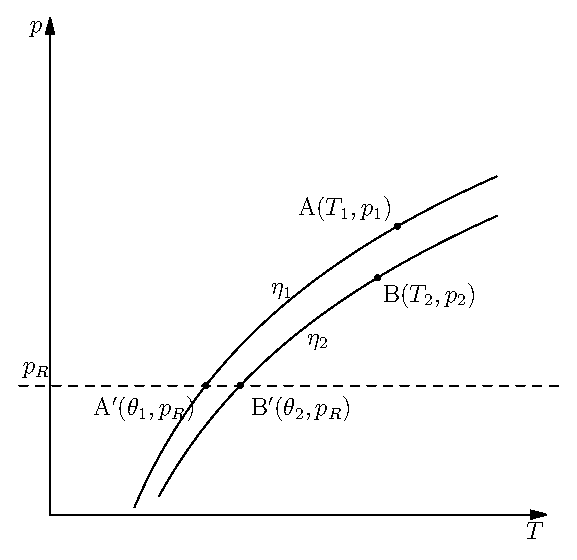
\includegraphics[width=\linewidth]{./appendix_Fig1}
\caption{\footnotesize 状態 A から状態 B に変化したときのエントロピーの微小変化$d\eta (= \eta_2-\eta_1)$を考える.}
\label{fig:appendix_Fig1}
\end{wrapfigure}
% % % % % % % % % % % % % % % % % % % % % % % % % %
エントロピーの変化と\eqref{eq:PTemp_generalDef}で定義される温位の変化の関係式の導くために, 
任意の状態$(T_1,p_1)$から任意の状態$(T_2,p_2)$に変化したときのエントロピーの微小変化$d\eta$を考えよう.
それぞれの状態は, 図\ref{fig:appendix_Fig1}において点 A, B に対応している. 

エントロピーを温度と圧力の関数とするとき, その微小変化は, 
\begin{equation*}
 (d\eta)_{{\rm A}\to{\rm B}} = \DP[][T]{\eta}{p} (dp)_{{\rm A}\to{\rm B}} + \DP[][p]{\eta}{T} (dT)_{{\rm A}\to{\rm B}}
\tag{A.1}
\end{equation*}
と書ける. 
添字${\rm A}\to{\rm B}$は, 状態 A から状態 B へ変化したときの微小変化であることを示している. 
エントロピーと温位の微小変化の関係式を導くには, (A.1) の右辺の
$(dp)_{\rm A \to B}, (dT)_{\rm A \to B}$を, \eqref{eq:PTemp_generalDef}の定義を使って$(d\theta)_{\rm A \to B}$に
書き換えなければならない.  
もし, 実直に\eqref{eq:PTemp_generalDef}の両辺の変分をとることにより 
\eqref{eq:ptemp_entropy_relation_ingeneral}を導くならば, やや複雑な計算が必要である%
\footnote{
\eqref{eq:PTemp_generalDef}の両辺の変分をとることにより 
\eqref{eq:ptemp_entropy_relation_ingeneral}を導く場合を考えよう. 

$T,p$を独立変数として\eqref{eq:PTemp_generalDef}の両辺の変分を取り, 変形すれば, 
\begin{align*}
 dT = \left[ d\theta + \DP[][\eta]{T}{p} dp \right] \left[ 1 + \int_{p}^{p_R}  \DP{}{T} \DP[][\eta]{T}{p^\prime} (T,p^\prime) dp^\prime \right]^{-1} 
\end{align*}
を得る. 
積分を含む因子を$I(p,T,p_R)$で表して, (A.1) の右辺に代入し整理すれば, 
\begin{align*}
 d\eta &= I\DP[][p]{\eta}{T} \; d\theta 
        + \left[ \DP[][T]{\eta}{p} + I \DP[][p]{\eta}{T} \DP[][\eta]{T}{p}  \right] dp  \\
       &= I \DP[][p]{\eta}{T} \; d\theta 
        + \left[ \left( 1-I \right)\DP[][T]{\eta}{p} \right] dp. 
\end{align*}
後は本文と同様の議論をすれば良い. 
なお, $p=p_R$の圧力一定の過程では$I=1$となることに注意されたい. 
}. 
代わりに, 次のように考えるとエントロピーと温位の微小変化の関係式を簡単に導ける. 

点 A, B 間のエントロピーの変化を,
代わりに$p=p_R$上の点 A$^\prime$, B$^\prime$間で考えることにしよう. 
点 A$^\prime$, B$^\prime$間で圧力一定の過程を考えるとき, 
その過程における温度は定義により温位である. 
したがって, 
点 A$^\prime$, B$^\prime$間のエントロピーの微小変化は, 
\begin{equation*}
 (d\eta)_{{\rm A^\prime}\to{\rm B^\prime}} = \dfrac{c_p(p_R,\theta)}{\theta} (d\theta)_{{\rm A^\prime}\to{\rm B^\prime}}
\tag{A.2}
\end{equation*}
と書ける. 
ただし, 定圧比熱の定義を用いた. 
また, 点 A$^\prime$, B$^\prime$はそれぞれ, 点 A, Bと同じ等エントロピー線$\eta_1, \eta_2$上にあるので, 
$(d\eta)_{\rm A \to B} = (d\eta)_{\rm A^\prime \to B^\prime}, \;
(d\theta)_{\rm A \to B} = (d\theta)_{\rm A^\prime \to B^\prime}$
が成り立つ. 
したがって,  
\begin{equation*}
 (d\eta)_{\rm A\to B} = \dfrac{c_p(p_R,\theta)}{\theta} (d\theta)_{\rm A \to B}
\tag{A.3}
\end{equation*}
を得る. 



\end{document}
%%
%%%%%%%%              Text End                  %%%%%%%%
%%%%%%%%%%%%%%%%%%%%%%%%%%%%%%%%%%%%%%%%%%%%%%%%%%%%%%%%
